\subsubsection*{Cost Category 22.01.06: Vacuum System}

The vacuum system in a nuclear fusion reactor plays a critical role in creating and maintaining a high-quality vacuum environment essential for plasma containment and fusion reactions. It comprises various components such as vacuum vessels, primary and roughing vacuum pumps, helium liquefier-refrigerators, and vacuum ducts, each contributing to the effective evacuation and thermal management necessary for sustained and controlled fusion processes. Cost Category 22.1.6 Vacuum System consists of:  

\begin{itemize}
\item 22.01.06.01 Vacuum Vessel.  The vacuum vessel is a sealed container designed to maintain a high vacuum environment, essential for minimizing interactions between the plasma and any residual gases, thus enabling controlled fusion reactions.

\item 22.01.06.02 Helium Liquefier-Refrigerators. Helium liquefier-refrigerators are used to cool components of the reactor, such as superconducting magnets, to extremely low temperatures, often necessary for maintaining superconductivity and efficient thermal management.

\item 22.01.06.03 Primary Vacuum Pumps. Primary vacuum pumps are responsible for creating and maintaining the vacuum within the vessel by removing gases and air, which is crucial for the initial establishment of the vacuum environment.

\item 22.01.06.04 Roughing or Backing Pumps. Roughing or backing pumps are used in conjunction with primary vacuum pumps, typically to provide the initial evacuation of the vessel and reduce the pressure to a level where primary pumps can operate effectively.

\item 22.01.06.05 Vacuum Ducts. Vacuum ducts are the conduits that connect various components of the vacuum system, facilitating the efficient transport and removal of gases from the vacuum vessel to the pumps.
\end{itemize}

Each subsystem is considered in detail as follows. \\
%(see \ref{tab:subsystem_cost_plainvars})

22.01.06.01 Vacuum vessel: this account dominates the cost of the vacuum system and includes only the structural elements of the vacuum system, including the main vacuum vessel chamber, port enclosures, the vacuum door assembly, bulk shielding inside the walls of the vacuum vessel and any manifold / padding \cite{waganer2006design}. It serves two primary functions: (1) to maintain the vacuum environment created by the pumping system for the plasma experiments; (2) to provide the structural support for the superconducting magnets and the other internal and external systems. The design for this mirror concept is based on the vessel used for the MFTF-B at LLNL \cite{gerich1986design}. \\

The vacuum vessel serves as a  key structural element in the reactor, from which other systems including and cryogenic systems are mounted.  As such, there are several key loading requirements:

\begin{itemize}
    \item Gravity load. The vessel must support the 1 g force acting straight down on the entire vessel and the components it supports. The dominant masses are the vessel itself massstruct tonnes, the total coil mass COILM tonnes, and auxiliary components inside and outside the vessel, $\sim$500 tonnes.

    \item External pressure load. The external pressure load is caused by the standard atmospheric pressure acting on the vessel shell when the vessel is under vacuum, plus an additional 10\% of the atmospheric load to account for magnetic  pressure on the shell resulting from the sudden collapse of the magnetic field. 

    \item Thermal cooldown load. The thermal cooldown load is  caused by the magnets cooling to 4 K, while the vessel remains at room temperature. Because the magnets are connected to the vessel by a number of support struts on each  magnet group, the possibility exists for an over-constrained  strut system to generate thermal contraction loads.

    \item Environmental thermal load. The environmental thermal load is caused by the variation in the air temperature surrounding the vessel.

\end{itemize}

For the chamber geometry specified in Cost Category 22.01.02, a total material volume of materialvolume m$^3$ is calculated. ASTM A240 Type-304 stainless steel is used because it is nonmagnetic, has good fracture toughness and welding properties, is readily available and inexpensive, and a total mass of massstruct tons is required, costing vesmatcost M USD. Considering the manufacturing and assembly process, however, will increase the vessel cost significantly. One notable requirement is to polish the entire inner surface to maintain the required high vacuum, and reduce the risk of electrical faults. An approximate manufacturing factor of vesmfr is assumed for the entire process. This results in a cost for vacuum vessel of C22010601 M USD.\\

\begin{table}[h]
    \centering
    \resizebox{0.4\linewidth}{!}{%
    \begin{tabular}{lc}
    \hline
        Vessel volume (m$^3$) & vesvol\\
        Material volume (m$^3$) & materialvolume\\
        Material & ASTM A240 304 SS\\
        Material mass (tons) & massstruct\\
        Material cost (M USD) & vesmatcost\\
        Total cost (M USD) & C22010601 \\
         \hline
    \end{tabular}}
    \caption{Vacuum vessel parameters.}
    \label{tab:ves_params}
\end{table}






22.01.06.02 Helium Liquefier-Refrigerators: This subsystem is the helium refrigeration and liquefaction process equipment. It is responsible for supplying the cooling necessary to maintain an operation temperature of 20 K at coils, absent in this case. \\

The costs for this subsystem are C22010601 M USD for the vacuum vessel, C22010602 M USD for the cooling systems, C22010603 M USD for the vacuum pumping systems, and C22010604 M USD for the roughing pump. The total cost is C220106 M USD.\\

%To determine the cooling power necessary to maintain 20 K in the coils, an analytical approach is taken, considering the primary heating components at the HTS coils. These are assumed to be the heat conducted through the support structure, and the neutron flux through the blanket (assuming 99\% of the neutron power is captured in the blanket). At 20 K, for one coil, these are estimated to contribute 11.2 and 1.8 kW, respectively. Scaling for a refrigeration efficiency of 15\% of the Carnot efficiency between 300 and 20 K, this results in a room temperature cooling power requirement of Qin MW. The operation temperature is selected based on a trade-off of the cooling efficiency (see fig \ref{fig:cool_eff}), and the superconducting properties of the HTS coils.\\

%Using STARFIRE as a reference (ITER cryogenic costs seem to be unexpectedly high), the cost for 20 kW of cooling at 4.2 K is 25.2 M USD. Scaling this to the cooling requirements of the system presented here results in a cost of C22010602 M USD. \\

%\begin{figure}[h]
%    \centering
%    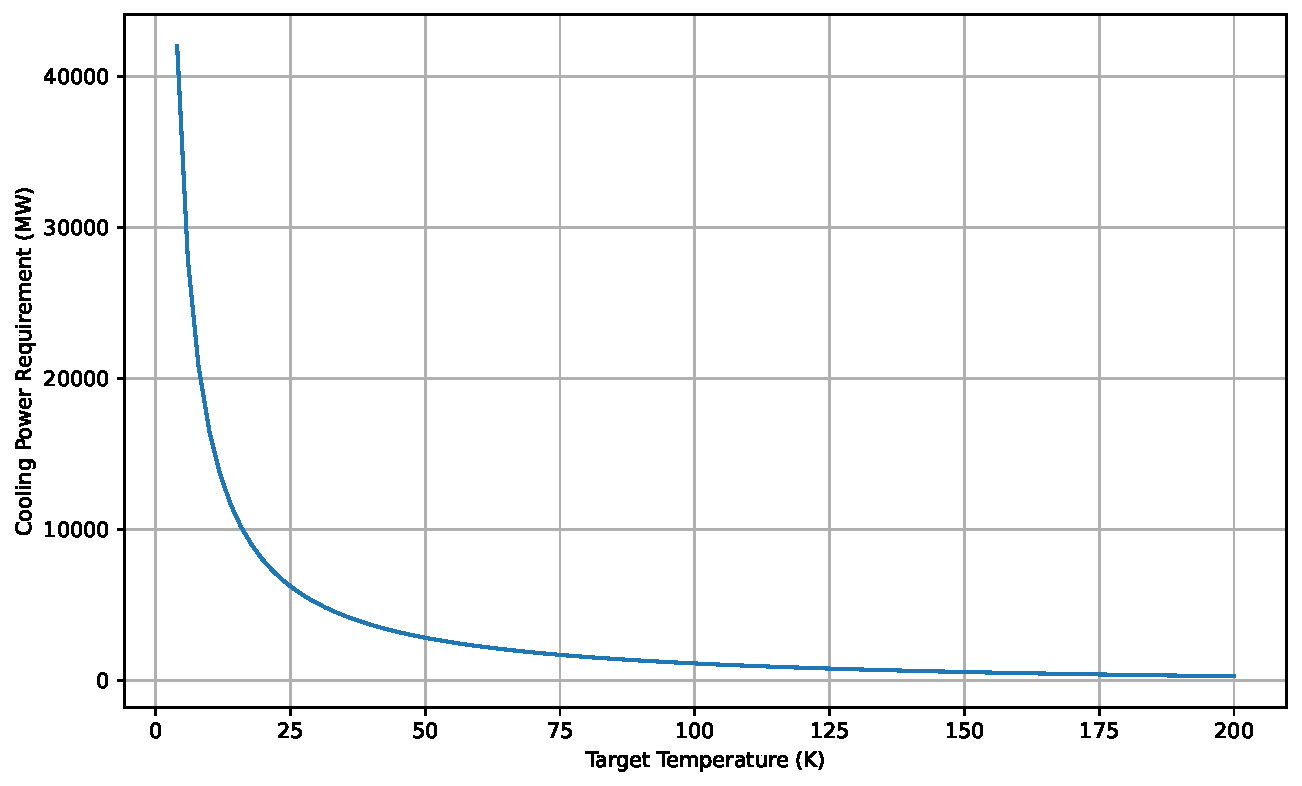
\includegraphics[width=0.75\linewidth]{Figures/cooling_efficiency.pdf}
%    \caption{The cooling power requirement for various magnet operating temperatures.}
%    \label{fig:cool_eff}
%\end{figure}



22.01.06.03 Primary Vacuum Pumps: consists of d a distributed vacuum subsystem with vacuum pumps located at each sector. For a vacuum of vesvol m$^3$, novpumps vacuum pumps will be required, costing 50 K USD each, corresponding to a total pumping system cost of C22010603 M USD.\\

22.01.06.04 Roughing Pumps: Consists of a single roughing pump to establish an initial vacuum and will cost C22010604 M USD.

